\chapter{കേരളത്തിൽ റാണിമാർ ഉണ്ടായിരുന്നോ?}
\label{chapter3}
\begin{figure}[h]
\begin{center}
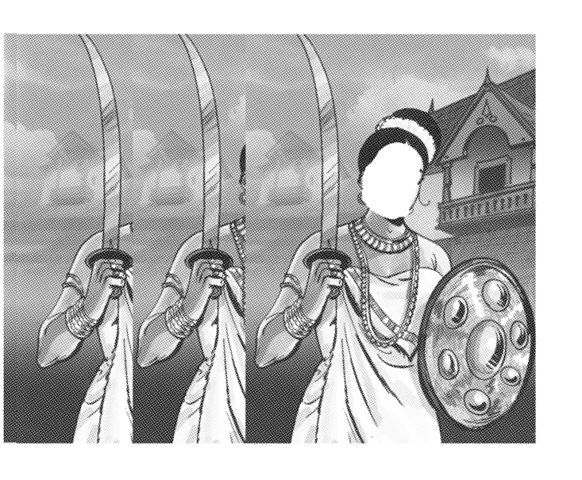
\includegraphics[width=\textwidth,height=7cm]{Kulasthree_Chapter_three_pic01.jpg}
\end{center}
%\caption*{പുലയർ - കെ പി പത്മനാഭ മേനോൻ - വാള്യം 3, (1929), 1984}
\end{figure}

\paragraph{}പഞ്ചായത്തുകളിലെ സ്ത്രീസംവരണം 33ൽനിന്ന് 50 ശതമാനമായി ഉയർന്നിരിക്കുന്ന ഇന്നത്തെക്കാലത്തും കേരളരാഷ്ട്രീയത്തിന്റെ ഉന്നതങ്ങളിൽ വളരെക്കുറച്ചു സ്ത്രീകളേയുള്ളു. എളിയ മട്ടിൽ ജനസേവനം നടത്തുന്ന സ്ത്രീകളോട് നമുക്കു വളരെ പ്രിയമാണ്. എന്നാൽ അധികാരരാഷ്ട്രീയത്തിൽ പ്രവേശിക്കാൻ ശ്രമിക്കുന്ന സ്ത്രീകളെ അല്പമൊരു പുച്ഛത്തോടെയാണ് നാം കാണുന്നത്. 'പൗരുഷക്കാരി,' 'തന്റേടി' മുതലായ വിശേഷണങ്ങളാണ് നാം അവർക്കു നൽകാറുള്ളത്! പുരുഷന്മാർക്ക് രാഷ്ട്രീയാധികാരത്തെ മൊത്തത്തിൽ തീറെഴുതിക്കൊടുക്കുന്ന ഈ രീതി എങ്ങനെയാണ് രൂപപ്പെട്ടത്? മലയാളികളുടെ പരമ്പരാഗത രാഷ്ട്രീയസ്ഥാപനങ്ങളിൽ - രാജസ്വരൂപങ്ങളിൽ - ആ സ്ഥാനങ്ങളിലെത്തിയ സ്ത്രീകൾക്ക് ചില സാദ്ധ്യതകളുണ്ടായിരുന്നുവെന്നും ക്രമേണ അവ നഷ്ടമാവുകയാണുണ്ടായതെന്നും നാം തിരിച്ചറിയേണ്ടതുണ്ട്.

\paragraph{}ആമുഖത്തിൽ പറഞ്ഞ കാര്യങ്ങളുടെ വെളിച്ചത്തിൽ ഈ ചോദ്യത്തിന് വലിയ പ്രാധാന്യം കൊടുക്കേണ്ടതില്ലെന്ന് നമുക്ക് വാദിക്കാവുന്നതാണ്. നമ്മുടെ ഭൂതകാലം ചികഞ്ഞുനോക്കിയാൽ ഒന്നോ രണ്ടോ കഴിവുറ്റ റാണിമാരെ കണ്ടെത്താൻ കഴിയും. പക്ഷേ, ആ കണ്ടെത്തലിൽനിന്ന് നമുക്കെന്താണു ഗുണം? നേരത്തേ പറഞ്ഞതുപോലെ, ഒരു ഉണ്ണിയാർച്ചയെ കണ്ടെത്തിയെന്നു കരുതി അന്നത്തെ ഇവിടത്തെ പെണ്ണുങ്ങൾ മുഴുവൻ കളരിപഠിച്ച അഭ്യാസികളായിരുന്നുവെന്ന് പറയാൻപറ്റുമോ? പറ്റില്ല, തീർച്ച! അതുപോലെ, ഒന്നുരണ്ട് നല്ല ഭരണാധികാരിണികളെ കണ്ടെത്തിയെന്നു കരുതി അന്നത്തെ മേലാളസ്ത്രീകൾക്ക് ഭരണാധികാരത്തിൽ പുരുഷനുതുല്യമായ നിലയുണ്ടായിരുന്നുവെന്ന് വാദിക്കാൻ കഴിയില്ല. ഒന്നാമത്, റാണിമാരെ സാധാരണസ്ത്രീകളുടെ കൂട്ടത്തിൽപെടുത്താൻപറ്റില്ല. അവർ ഉന്നതജാതിക്കാരും കുടുംബക്കാരുമായിരുന്നു. രണ്ടാമത്, ഒന്നുരണ്ടുദാഹരണങ്ങൾ തിരഞ്ഞുപിടിക്കുന്നതുകൊണ്ട് സ്ത്രീ പുരുഷനു തുല്യയായിരുന്നുവെന്ന് സമർത്ഥിക്കാനാവില്ല - ഏതു സമൂഹത്തിലും പുരുഷനൊപ്പം നിൽക്കുന്ന ഒന്നുരണ്ട് അസാമാന്യസ്ത്രീകൾ ഉണ്ടാകുമെന്ന മറുപടിയായിരിക്കും കിട്ടുക.
\paragraph{}എങ്കിലും പഴയ മലയാളിസമൂഹത്തിന്റെ ഏറ്റവും ഉയർന്നതട്ടുകളിലെ സ്ത്രീകളുടെ അനുഭവമെന്തായിരുന്നുവെന്ന് അന്വേഷിക്കുന്നത് സ്ത്രീകളെ മൊത്തത്തിൽ ബാധിച്ച ചില വൻസാമൂഹ്യമാറ്റങ്ങളിലേക്ക് കൂടുതൽ വെളിച്ചംവീശും. കേരളത്തിൽ ഇന്നും സ്ത്രീകൾക്ക് അധികം പ്രവേശനമില്ലാത്ത ഒരു മേഖലയാണ് അധികാരരാഷ്ട്രീയം. പല പരീക്ഷണങ്ങളും നടത്തിയിട്ടും രാഷ്ട്രീയത്തിന്റെ ഉന്നതമേഖലകളിലേക്ക് അധികം സ്ത്രീകൾ കയറിച്ചെന്നിട്ടില്ല. കയറിച്ചെന്ന ചിലർക്കു കിട്ടിയ സ്വീകരണം ഒട്ടും ആശാവഹവുമായിരുന്നില്ല. (ഇടതുപക്ഷപ്രസ്ഥാനത്തിലൂടെ നേതൃത്വനിരയിലേക്കുയർന്ന കെ.ആർ. ഗൗരിയമ്മയുടെ അനുഭവം ഓർമ്മിക്കുക) കേരളത്തിലെ റാണിമാരുടെ ചരിത്രം ഇതെങ്ങനെ സംഭവിച്ചു എന്നതിനെക്കുറിച്ച് ചില സൂചനകൾ നൽകുന്നു.
\paragraph{}ഒന്നുരണ്ട് അസാമാന്യസ്ത്രീകൾ കേരളത്തിന്റെ കഴിഞ്ഞ കാലത്തിലുമുണ്ട്. അവരിൽ പ്രധാനിയാണ് പതിനേഴാം നൂറ്റാണ്ടിൽ തെക്കൻകേരളത്തിൽ (പിൽക്കാലത്തെ തിരുവിതാകൂർ) ജീവിച്ചിരുന്ന അശ്വതിതിരുനാൾ തമ്പുരാട്ടി. സ്ത്രീകൾ മൂപ്പുവാണ സ്വരൂപമെന്ന പേരിൽ - അതായത്, ഏറ്റവും മൂത്തസ്ത്രീ കാരണവത്തിയും ഭരണാധികാരിയുമായി വാണിരുന്ന സ്വരൂപം എന്ന പേരിൽ - അറിയപ്പെട്ടിരുന്ന ആറ്റിങ്ങൽ സ്വരൂപത്തിലെ മൂത്ത തമ്പുരാട്ടിയായിരുന്നു ഇവർ. ഉമയമ്മറാണി എന്ന പേരിൽ ഇവർ പ്രസിദ്ധയാണ്. 1678 മുതൽ 1698 വരെയായിരുന്നു ഇവരുടെ ഭരണകാലം. തിരുവനന്തപുരത്തെ പഴമക്കാർ ഉമയമ്മറാണിയെക്കുറിച്ചുളള പല കഥകളും കേട്ടിരിക്കും. കളിപ്പാങ്കുളം എന്ന സ്ഥലത്തുവച്ചുണ്ടായ ദാരുണസംഭവത്തെക്കുറിച്ചായിരിക്കാം അധികംപേരും കേട്ടിരിക്കുക. ഉമയമ്മറാണിക്ക് ആറ് ആൺമക്കളുണ്ടായിരുന്നെന്നും കളിപ്പാങ്കുളത്തിൽ നീന്താനിറങ്ങിയ കുമാരന്മാരെ ദുഷ്ടന്മാരായ മാടമ്പിമാർ കൊന്നുകളഞ്ഞുവെന്നുമാണ് കഥയുടെ രത്നച്ചുരുക്കം. പിൽക്കാലത്ത്, ഇരുപതാംനൂറ്റാണ്ടിന്റെ ആദ്യപകുതിയിൽ മലയാളകവിതയ്ക്കു പുതുജീവൻ പകർന്ന മൂന്നു കവികളിൽ (ആധുനികകവിത്രയമെന്നാണ് അവരെ വിശേഷിപ്പിച്ചിട്ടുളളത്) ഒരാളായിരുന്ന ഉള്ളൂർ എസ്സ്. പരമേശ്വരയ്യർ ഈ കളിപ്പാങ്കുളംകഥയെ ഉമാകേരളം (1913) എന്ന തന്റെ മഹാകാവ്യത്തിൽ ഉപയോഗിച്ചു. തിരുവിതാംകൂറിനോടും കേരളത്തോടും കവിയുടെ ഭക്തി പ്രകടിപ്പിക്കുന്ന ഈ കാവ്യത്തിൽ ഉമയമ്മറാണി സാക്ഷാൽ കേരളത്തിന്റെ പ്രതീകമായി പ്രത്യക്ഷപ്പെടുന്നു. മക്കളുടെ ദാരുണമരണത്തിലും ധൈര്യംകൈവിടാത്ത, സുചരിതയായ വീരമാതാവായാണ് കവി അവരെ ചിത്രീകരിക്കുന്നത്. തിരുവിതാംകൂറിലെ മാടമ്പിമാരുടെ ദുർഭരണവും വിദേശീയാക്രമണവുമെല്ലാം ചേർന്നുണ്ടായ പ്രതിസന്ധിയിൽനിന്ന് നാടിനെ രക്ഷിക്കാൻ പണിപ്പെടുന്ന മഹതിയായ മാതാവായിട്ടാണ് അവർ ആ കൃതിയിൽ നിറഞ്ഞുനിൽക്കുന്നത്. അവർക്ക് ഒടുവിൽ സിദ്ധിക്കുന്ന വിജയം കേരളത്തിന്റെതന്നെ വിജയമാകുന്നു.
\paragraph{എന്നാൽ ഉമാകേരളത്തിലെ ഉമയമ്മയ്ക്ക് ചരിത്രരേഖകളിൽ പ്രത്യക്ഷപ്പെടുന്ന ഉമയമ്മറാണിയുമായി വലിയ സാമ്യമൊന്നുമില്ലെന്നതാണ് കൗതുകകരമായ കാര്യം. ഉള്ളൂർ കവിമാത്രമായിരുന്നില്ല, അറിയപ്പെട്ട ചരിത്രഗവേഷകൻകൂടിയായിരുന്നു. അദ്ദേഹംതന്നെ തന്റെ ചരിത്രപഠനത്തിൽ കളിപ്പാങ്കുളം സംഭവം നടന്നതായി തെളിവില്ലെന്ന് സൂചിപ്പിക്കുന്നുണ്ട്. ആറെണ്ണംപോയിട്ട് ഒരു സന്താനംപോലും ഉമയമ്മയ്ക്കില്ലായിരുന്നെന്നും അവർ പ്രസവിച്ചതായിപ്പോലും അറിവില്ലെന്നും പിൽക്കാലത്തുണ്ടായ ചരിത്രപഠനങ്ങൾ അവകാശപ്പെടുന്നു. ഇവിടെ യൂറോപ്യർ - ലന്തക്കാരും ബ്രിട്ടിഷുകാരും - തങ്ങളുടെ ആധിപത്യമുറപ്പിക്കാൻ കിണഞ്ഞു ശ്രമിച്ചിരന്ന പതിനേഴാംനൂറ്റാണ്ടിന്റെ അവസാനമായിരുന്നു ഉമയമ്മറാണി ഭരണമേറ്റത്. അവർ ബാക്കിവച്ച പല രേഖകളിലും ഉമയമ്മറാണിയെക്കുറിച്ചുള്ള ചിത്രങ്ങളുണ്ട്. ഈ വിവരങ്ങളെ ഏറെക്കുറെ സ്ഥിരീകരിക്കുന്ന ഐതിഹ്യങ്ങളും പ്രചാരത്തിലുണ്ട്.
}

\paragraph{}ആറ്റിങ്ങൽസ്വരൂപത്തിന്റെ മൂത്ത തമ്പുരാട്ടിയായി അവർ 1678ൽ സ്ഥാനമേറ്റു. അന്നത്തെ അധികാരരാഷ്ട്രീയമെന്നുവച്ചാൽ തെക്കൻകേരളത്തിലുണ്ടായിരുന്ന രാജസ്വരൂപങ്ങൾ തമ്മിലുള്ള മത്സരമായിരുന്നു. തൃപ്പാപ്പൂർ, ദേശിങ്ങനാട്, ഇളയിടത്തു സ്വരൂപം മുതലായ നിരവധി രാജസ്വരൂപങ്ങൾ തമ്മിൽ വലിയ മത്സരംനടന്ന കാലം. ഈ മത്സരത്തിൽ ഉമയമ്മറാണി കാര്യമായി പങ്കെടുത്തിരുന്നുവെന്നാണ് രേഖകളിൽ കാണാനുള്ളത്. ആറ്റിങ്ങലിൽ മാത്രമല്ല അവിടംകടന്നു അക്കാലെത്ത മറ്റു സ്വരൂപങ്ങളിലും തന്റെ സ്വാധീനമുറപ്പിക്കാൻ അവർ ശ്രമിച്ചുവെന്ന് ചരിത്രരേഖകൾ വ്യക്തമാക്കുന്നു. ഉദാഹരണത്തിന് അന്നത്തെ തിരുവിതാംകൂറിൽ (അന്ന് ആറ്റിങ്ങൽ തിരുവിതാംകൂറിൽനിന്ന് വേറിട്ടായിരുന്നു) ഉമയമ്മറാണി ആറ്റിങ്ങൽ മൂത്തതമ്പുരാനായിട്ട് അധികം കഴിയുന്നതിനുമുമ്പ് തിരുവിതാംകൂർ രാജാവായിരുന്ന ആദിത്യവർമ്മ അന്തരിച്ചു. തുടർന്നുണ്ടായ പിന്തുടർച്ചാത്തർക്കത്തിൽ അവർ ശക്തമായി ഇടപെടാൻ ശ്രമിച്ചു. തന്റെ താൽപര്യമനുസരിച്ച് ഒരാളെ രാജാവായി അവിടെ വാഴിക്കാൻ പരിശ്രമിച്ചു. ഒടുവിൽ അവർ ദത്തെടുത്ത പുറവഴിനാട് കേരളവർമ്മ തിരുവിതാംകൂർ രാജാവാകുകയും ചെയ്തു. എന്നാൽ അവർതന്നെ പിൽക്കാലത്ത് ഈ വ്യക്തിക്ക് എതിരാവുകയും അയാളെ കൊന്നുകളയാനുള്ള ഗൂഢാലോചനയിൽ പങ്കുചേരുകയും ചെയ്തുവെന്നാണ് എഴുതപ്പെട്ട ചരിത്രരേഖകളും വാമൊഴിയായി പ്രചരിച്ച കഥകളും പറയുന്നത്. 1692ൽ ഇയാൾ കൊല്ലപ്പെട്ടു. ഉമയമ്മറാണി തിരുവനന്തപുരത്തെ ശ്രീപത്മനാഭസ്വാമിക്ഷേത്രത്തിലും തന്റെ സ്വാധീനമുറപ്പിക്കാൻ ശ്രമിച്ചതായി തെളിവുണ്ട്. ബ്രിട്ടിഷ് പ്രതിനിധികളുമായി നേരിട്ട് ചർച്ചകളിലേർപ്പെടാനും അവരെ സ്വാധീനിച്ച് തന്റെ അധികാരമുറപ്പിക്കാനും അവർ ഒട്ടും മടിച്ചിരുന്നില്ല. ബ്രിട്ടിഷുകാർക്ക് ആദ്യമായി കച്ചവടസ്ഥാപനം അനുവദിച്ചത് അവരായിരുന്നു. ദത്തെടുക്കപ്പെട്ട കേരളവർമ്മയെ അവർ തിരുവിതാംകൂർ രാജസ്ഥാനത്തെത്തിച്ചത് നടപ്പിലുണ്ടായിരുന്ന പിന്തുടർച്ചാനിയമങ്ങളെ ലംഘിച്ചുകൊണ്ടത്രെ. ചുരുക്കിപ്പറഞ്ഞാൽ, അന്നത്തെ രാഷ്ട്രീയ അധികാരക്കളിയുടെ പതിനെട്ടടവും പാച്ചിലും വശത്താക്കിയ, എല്ലാത്തരം രാഷ്ട്രീയകൗശലങ്ങളും വശമായിരുന്ന, രാഷ്ട്രീയാധികാരം ആത്മവിശ്വാസത്തോടെ കൈകാര്യംചെയ്തിരുന്ന ഒരു റാണിയുടെ രൂപമാണ് ചരിത്രരേഖകളിൽ തെളിയുന്നത്. അധികാരത്തിനുവേണ്ടി ആചാരത്തെ അതിലംഘിക്കാൻ മടിക്കാത്ത ഒരുവൾ. ആറ്റിങ്ങൽ തമ്പുരാട്ടിമാരെയും ഉമയമ്മയെയും നേരിൽക്കണ്ട ഒരു യൂറോപ്യൻ സൈനികൻ 1677ൽ അവരെ ഇങ്ങനെ വിവരിക്കുന്നു:

\begin{quote}
ആറ്റിങ്ങൽ റാണി തിരുവിതാംകൂറിന്റെ മാതൃഗൃഹമാണ്; മാത്രമല്ല, തൃപ്പാപ്പൂർസ്വരൂപത്തിന്റെ മൂപ്പും വഹിക്കുന്നു. തിരുവിതാംകൂറിൽനിന്നു സ്വതന്ത്രമായി നിൽക്കുന്ന വലിയൊരു ഭൂപ്രദേശവും അവർക്ക് സ്വന്തമായുണ്ട്. മൂത്ത തമ്പുരാട്ടിക്കൊപ്പം ഒരു ഇളയ തമ്പുരാട്ടിയുമുണ്ട്. പൗരുഷവും കുലീനതയും തികഞ്ഞ അവരെ എല്ലാവർക്കും ഭയവും ബഹുമാനവുമാണ്. അവരുടെ സ്ത്രീത്വത്തെ ചിലർ ബഹുമാനിക്കുന്നു. മറ്റുചിലർ മൂത്ത തമ്പുരാട്ടിയോടുളള ബഹുമാനംകൊണ്ട് അവരെ വന്ദിക്കുന്നു. ഇങ്ങനെ കിട്ടുന്ന ആദരവിനെ തനിക്കനുകൂലമായി ഉപയോഗിക്കാൻ ഈ ഇളയ തമ്പുരാട്ടിക്ക് നല്ല കഴിവാണ്. അതിലൂടെ അവർ ആറ്റിങ്ങൽ മാത്രമല്ല, തിരുവിതാംകൂർതന്നെ ഭരിക്കുന്നു. അവിടത്തെ ആചാരപ്രകാരം തിരുവിതാംകൂറിലേക്ക് തമ്പുരാട്ടിമാർ കാലെടുത്തുവച്ചുകൂടാത്തതാണ്. കരമനയാറു കടന്നാൽ കളങ്കമുണ്ടാകുമെന്നാണ് വിശ്വാസം. എന്നാൽ ഈ പൗരുഷക്കാരി ആ മാമൂൽ അടുത്തകാലത്ത് ലംഘിച്ചു. രാജാവുപോലും അവരുടെ മുന്നിൽനിന്ന് പറപറക്കുന്നു.
(ശിവശങ്കരൻ നായർ, എ ഹാൻഡ് ബുക് ഓഫ് കേരള, വാല്യം.1, തിരുവനന്തപുരം 2001, പുറം 144)
\end{quote}



